%!TEX root = thesis-kdyoung.tex

\chapter{Theoretical Background} \label{chap:theory}
In this chapter we provide the theoretical background needed
for the work presented in the following chapters.
As such, we give summaries of the relevant literature from
four fields spanning mathematics and computer science.
These include background knowledge of the problem of assembly
line balancing (Sect. \ref{sec:lit:ALB}); modelling and solving technology from the areas
of linear programming (Sect. \ref{sec:lit:mip}) and constraint programming (Sect. \ref{sec:lit:cp});
and lastly we delve into some of the recent
advances into the theory of Benders decomposition (Sect. \ref{sec:lit:bend}).

\section{Assembly Line Balancing}
\label{sec:lit:ALB}
Optimizing the construction of an assembly line to maximize or minimize 
some performance measure has been a problem of great interest to the 
research community since its introduction by Henry Ford
in 1915 \cite{Ford1922}.
Simply, it can be stated as a decision problem
where we seek optimal partition of work to assemble
a product.
The work must be divided
among discrete stations along a line (\eg conveyor belt),
while respecting a series of restrictions imposed by physical
limitations.
All variants of the \albp{} begin from this common starting point
and add further restrictions or considerations which
results in a range of generalizations.
We refer the interested reader to one of the surveys
of \authciteb{Baybars1986},
\authciteb{Becker2006} or
\authciteb{Boysen2007} for a detailed snapshot of
the problem's various extensions.

In this section we detail the basic version of the 
problem and the particular variant which
is relevant to our work.

\subsection{Simple Assembly Line Balancing Problem}
\label{sec:lit:SALBP}
The Simple Assembly Line Balancing Problem is the basic
type of the \albp{} \cite{Baybars1986,Scholl1999}.
It consists of a serial production line which produces a 
single product.
The tasks which need to be executed to achieve a product's completion
all have fixed processing times and all stations
along the line are uniform, \ie each is equivalently equipped
and manned by homogeneous workers or machines.

There are two primary parameters of the assembly line
which dictate the aim when solving the problem; these parameters
are the \emph{cycle time} and the number of stations, denoted
by $c$ and $m$ respectively.
We denote the \emph{load} of station $k$ by $l_k$, which is
defined as the sum of all processing times of tasks assigned to station
$k$.
The cycle time of an assembly line is defined as follows,
\[
	c=\max\{ \: l_k \:|\: k \in K \:\},
\]
\ie the largest load among all stations.
Physically, the cycle time of an assembly
line can be interpreted as how much time each station is given to work on a product,
before the product moves to the next station.
A lower cycle time means the conveyor belt can move faster and
products are output at a higher rate.

From the parameters $c$ and $m$, the \albp{} can be formulated as three 
different but highly related problems: type-1, type-2 and
type-E.
We now summarize each variety and its particular qualities in turn,
\begin{itemize}
	\item Type-1: Fixed $c$, variable $m$.\\[1pt]
	The type-1 variety, abbreviated as \sab{1} in the simple case, considers the
	cycle time to be fixed and the number of stations to be decided.
	This most commonly occurs when constructing a new assembly line.
	As an example, the \sab{1} is characterized using the classification
	scheme of  \authciteb{Boysen2007} by $[-|-|m]$.
	\item Type-2: Variable $c$, fixed $m$.\\[1pt]
	For the type-2 variety, the aim is to find the optimal cycle time given 
	that the number of stations along the line is fixed.
	In practice, this variety commonly corresponds to adapting an existing assembly line
	for a new purpose.
	\item Type-E: Variable $c$, variable $m$.\\[1pt]
	This variety deals with the case when both $c$ and $m$ are considered
	to be decision variables of the problem. Here, the objective
	is to optimize some measurement of line efficiency.
\end{itemize}

\subsection{Setup Assembly Line Balancing and Scheduling Problem}
\label{sec:lit:SUALBSP}
In this document, we are concerned with the SetUp Assembly Line Balancing and Scheduling Problem.
This variant differs from the basic \sab{} by introducing
sequence-dependent setup times between pairs of tasks
within a station's workload.
This type of consideration was first made in the literature by \authciteb{Andres2008}
in an attempt to reduce the gap between the existing academic theory
and the realities of assembly line problems posed by the industry.
In the problem tackled by \citeauthor{Andres2008},
they considered a setup time to exist between
a pair of consecutive tasks inside a station's sequence.
As such, it needed to be added to that station's
global processing time
and so these setup times directly affected
the cycle time of the line.
The authors considered heuristic rules and employed a Greedy
Randomized Adaptive Search Procedure (\grasp) to tackle the
type-1 version of the problem.
They also developed a lower-bound which was used
to estimate the quality of their solutions found.

Later, some of the same authors continued this work in
\authciteb{Martino2010}, where over 50 priority-rules were considered
for a heuristic procedure designed for the type-1 version.
All results found for the problem at this point in the 
literature indicated that adding these sequencing considerations
for the tasks made the problem much more difficult to solve.
This is demonstrated by only very small instances of the problem
being able to be optimally solved.

More recently, the work of \authciteb{Scholl2013} extended the previous
work on this problem and formally named it the \sua{}.
The \sua{} differs slightly from the problem tackled previously
by introducing a distinguishment between \emph{forward} and \emph{backward}
setup times.
The motivation for this differentiation is so the theoretical
problem can more accurately capture the physical aspects
of sequencing tasks.
A forward setup time occurs between two consecutive tasks assigned the same station,
if each task is processing the same item.
A backward setup time occurs between two consecutive tasks assigned the same station,
if each task is operating on different items on the assembly line.
Physically, a backward setup time captures the setup cost between the last task on the current
product and the first task on the next product.
We demonstrate this idea using 
a possible task sequence within two stations in Figure \ref{fig:lit:forwBackSetupExAbstractB}.
Forward setup times are denoted by $\phi$ and backward setup times
by $\beta$.

% \begin{figure}[H]
% 	\centering
% 	\caption{Setup times of a station's sequence (test A)}
% 	\vspace{2mm}
% 	\includegraphics[width=0.9\textwidth]{images/forwBackSetupExA.eps}
% 	\label{fig:lit:forwBackSetupExAbstractA}
% \end{figure}

\begin{figure}[tpb]
	\centering
	\caption{Setup times of a station's sequence}
	\vspace{2mm}
	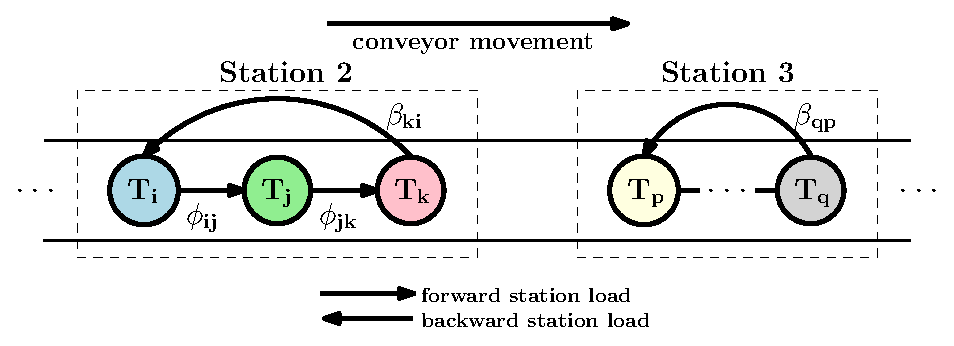
\includegraphics[width=0.9\textwidth]{images/forwBackSetupExB.eps}
	\label{fig:lit:forwBackSetupExAbstractB}
\end{figure}

% \begin{figure}[H]
% 	\centering
% 	\caption{Setup times of a station's sequence (test C)}
% 	\vspace{2mm}
% 	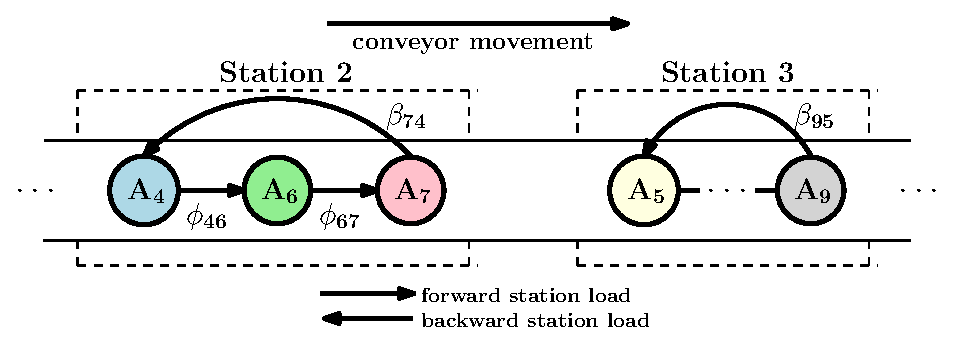
\includegraphics[width=0.9\textwidth]{images/forwBackSetupExC.eps}
% 	\label{fig:lit:forwBackSetupExAbstractC}
% \end{figure}

\authciteb{Scholl2013} proposed an exact solution approach by a
mathematical formulation of the type-1 problem as a mixed integer program.
Using the scheme of \authciteb{Boysen2007},
the \sua{1} can be formally classified as,
\[	\text{\sua{1}: }[\Delta t_{dir}|-|m].	\]
Further to their mathematical model, a range of tools were proposed which could be composed
in a number of ways to create new heuristic approaches for the problem.

\authciteb{Esmaeilbeigi2016} give the most recent contribution of the literature
to the study of the \sua{}.
In their paper, three new mixed-integer formulations are presented of the \sua{1}
which are based on different ways of representing the decisions.
Their first two formulations are station-based and the last is a purely
scheduling-based formulation which has abstracted the
assignment decisions away from the problem.
Each of the three models presented are also modified to be suited
to the type-2 version of the \sua{}.
Although these models were presented, the type-2 problem
was not the authors primary concern and as such the models were not tested.

In the literature there have been few attempts to tackle the type-2 variety of the \sua{}.
The first was by \authciteb{Yolmeh2012} who use a Genetic Algorithm
which is applicable to either the type-1 case or type-2 case.
The only other approaches to the type-2 problem
which have been explored are the three mixed integer programs
mentioned earlier from \authciteb{Esmaeilbeigi2016}.

\section{Mixed Integer Programming}
\label{sec:lit:mip}
A Mixed Integer Program is a common extension of the fundamental
Linear Program (LP) of the Operations Research discipline.
MIPs present the additional constraint on some of their decision
variables that restrict their domain to exclusively integer values.
Problems which require integer valued solutions occur in many
real-world scenarios.
Example \ref{ex:lit:simpleMIP} presents a simple but quite
useful application of a problem with integer variables.

\begin{example}\label{ex:lit:simpleMIP}
	Consider assigning staff members to complete
	a given set of tasks.
	For a solution of this problem to be feasible we require that
	no fraction of any staff member is split across multiple tasks.
	Using continuous variables to model
	this problem will lead to invalid solutions and thus integer-valued
	variables are required. \qed
\end{example}

The flexibility of the mixed integer programming approach to modelling
problems has allowed MIPs to model a wide-range of optimization
problems.
A typical solution methodology when approaching a MIP is to
consider its linear relaxation.
This presents a much simpler problem to solve, but 
recovering a feasible integer solution from this relaxed problem
can prove challenging.

\subsection{Branch and Bound}
\label{sec:lit:mipBB}
The Branch and Bound (\bab) algorithm is a general tool which can
be applied to solve optimization problems which was first proposed by \authciteb{land1960}.
The structure of the method is general enough that it can be used
as a design paradigm for more involved ways of exploring the
solution space. As a result, it has spawned 
a variety of adaptations in the field of operations research since its
inception. Some of these include branch-and-cut (\authcite{Padberg1991}),
branch-and-price (\authcite{Savelsbergh1997})
and branch-and-infer (\authcite{Bockmayr1998}).
A procedure based on the \bab algorithm is the typical way of
approaching MIPs and so we now give an overview of
how this method operates.

The \bab method constructs a rooted tree used to explore the set of
all feasible solutions.
At a node of the tree, a decision variable is chosen as
the branching variable and the domain
of possible values for that variable is divided
between two child nodes.
The solution space of the current node is split
into two smaller disjoint subsets in these child nodes.
At the root of the tree, the solution space corresponds to all
possible feasible solutions to the original LP relaxation of the problem.
For each new node created by branching, the corresponding
relaxed LP is solved to determine the optimal
value at each node.
When each node is processed, a procedure called \emph{fathoming},
its optimal value is checked for both
integrality and feasibility.
If the node's solution is optimal and integer then it is compared to
the current best integer solution.
In a minimization (maximization) problem, if the new solution 
is less (more) than the current best, then 
the current best is replaced with the new optimal integer solution.
This new solution is called the incumbent.
Branching on the feasible solution space and solving each
relaxed sub-problems continues until all branches have been either
explored or are deemed unnecessary to explore, \ie \emph{pruned}.
At termination, the current incumbent solution is the optimal solution
to the original non-relaxed MIP, and thus the original problem
is solved.
We provide some pseudo-code of the \bab algorithm
for a minimization MIP in Algorithm \ref{alg:lit:bab}
in the Appendices.

\subsection{MIP Solver: \gurobi}
\label{sec:lit:mipGurobi}
\gurobi is a commercial solver designed for mathematical optimization problems including
LPs, quadratic programs (QPs) and MIPs.
Significant advances have been made to Gurobi's capabilities and other MIP solvers
during the last few decades due to a number of improvements
in the theory and computational hardware available \cite{Bixby2002}.
Some of the most important improvements in this area
are detailed in \authciteb{Lodi2010}.
These factors have given MIP solvers the ability to 
solve highly complex optimization problems while providing
a relatively easy to use interface for doing so.

To solve a MIP, Gurobi uses the branch-and-cut version
of the \bab algorithm.
Preprocessing is a common procedure implemented by solvers
where the problem's input to the solver is altered 
to remove obviously sub-optimal solutions from 
the solution space without removing any possibly optimal solution.
Further to this pre-solving step, there are numerous 
improvements made to the procedure of the \bab also.
Additional constraints called \emph{cutting planes}, or
simply \emph{cuts}, are added to the model
which do not remove any feasible solution but result in the linear relaxation
being closer to the non-relaxed problem's feasible solution space.
The feasible solution space of the original problem is
called the \emph{convex hull}.

Advances in the hardware over the past few decades
has been the other main source of improvement to solvers such as Gurobi.
Utilizing an algorithm which depends on branching the solution space
into disjoint subsets, has naturally favoured solvers such as Gurobi
by allowing them to take full advantage of parallel computing.
Currently, \gurobi can concurrently solve 1024 branches of
a \bab tree.
Taking advantage of this parallelization can provide
more than just a 1024-fold increase is computational power
due to the communication of solutions between branches.
For example, if one branch finds a high-quality integer feasible solution
then all other branches can immediately reap the benefits
by getting access to more effective pruning.

\section{Constraint Programming}
\label{sec:lit:cp}
Constraint Programming (CP) is a framework for modelling and solving optimization problems.
This framework has its roots in the field of Artificial Intelligence and the initial
conception of the idea is due to \authciteb{Jaffar1987},
who pointed out that the language PROLOG II is a special
case of a more general scheme: Constraint Logic Programming. 
CP uses a declarative descriptive of the problem by defining a set of decision variables
each with a set of possible values, \ie domains;
and a set of constraints which restrict the possible combinations of values for the
decision variables.

Over the past two decades, CP has been used extensively
to tackle a variety of combinatorial optimization problems.
The success of constraint programming can generally be attributed
to two of its unique features
\begin{enumerate}
	\item \emph{heterogeneous global constraints} which allow the user to write a high level
	model using the global constraints to capture important combinatorial structures.
	In most cases these constraints are formulated in such a way to be abstracted 
	away from the specific properties of any one problem.
	\item \emph{user-defined search} which allows the user to specify a structured
	search procedure for exploring the solution space, using their familiarity
	with the problem.
\end{enumerate}

CP has proven itself to be an effective solving technology
for many scheduling problems such as project \cite{Berthold2010}, 
train \cite{Rodriguez2007} and 
employee scheduling \cite{Demassey2005}
as well as other types of combinatorial problems such as bin packing \cite{Pisinger2007}.

We now provide short explanations of the features of CP mentioned above
and a description of the CP solver we chose to use, \chuffed.
To communicate with the solver, we chose to write our constraint
programs using the solver-independent CP language 
MiniZinc \cite{Nethercote2007}.
MiniZinc provides a vast library of global constraints
as well as an adequate search language.

\subsection{Global Constraints}
\label{sec:lit:cpGlob}
Global constraints are one of the powerful tools made available to us
when formulating constraint programs. They allow us to succinctly encode
complicated combinatorial structures that commonly occur among
discrete problems. One of the simpler, 
but highly applicable, global constraints is given in
Example \ref{ex:globCons}.

\begin{example}\label{ex:globCons}
	\aldif is a global constraint that takes an array of integer
	variables, each with a possibly different domain of possible values. This constraint
	simply requires all given variables to take different values in the solution. \qed
\end{example}

One drawback of global constraints is that each one must be individually
implemented in the solver. When posed by a problem with inherent combinatorial
structures, your choice of solver can be restricted as some solvers may
only partially support, or not support at all, the needed global constraints.
However the benefits of this type of constraint are not to be understated.
The fact that global constraints are formulated to be problem-agnostic can
provide users with much easier access to advances in the state-of-the-art solving technology.
To illustrate this point we consider the global constraint \cumu.

The \cumu global constraint was first introduced by \authciteb{Aggoun1993}
to efficiently solve and succinctly model a complex scheduling
problem.
Since then, the \cumu constraint has been widely used in a variety of problems
due to the fact that resources which are cumulatively restricted occur in many real-world problems.
A cumulatively restricted resource could represent a limited work force needed to execute a set
of tasks or a machine with a restriction on the number
of tasks it can run in parallel \cite{Schutt2011a}.

The \cumu constraint has commonly been applied to the Resource Constrained
Project Scheduling Problem (\RCPSP), which has many variants that 
are well-disposed to utilize the benefits of this global constraint.
Since its introduction, the \cumu constraint has had a number of improvements
proposed, some of these were by \authciteb{Caseau1994}, \authciteb{Nuijten1994},
\authciteb{Baptiste2000} and \authciteb{Carlier2004}. Each time an improvement
is made to \cumu~--- either by strengthening its propagation or by allowing it
to capture more varied and complex structures --- the results of all
problems where \cumu has previously been applied are improved as well.

% \begin{figure}[tbp]
% 	\centering
% 	\caption{Example of \cumu applied to a small cumulative resource problem {\color{red} (not complete)}}
% 	\includegraphics[width=0.95\textwidth]{images/cumu.png}
% 	\label{fig:examplePrecGraph}
% \end{figure}

By encoding the combinatorial nature of a problem using the global
constraints made available to us by CP, we are able to not
only take advantage of all the previous theoretical improvements to a global
constraint, but all future advances as well.

\subsection{User-Defined Search Procedures}
\label{sec:lit:cpSearch}
MiniZinc is a powerful modelling language for constraint programming
which is capable of concisely specifying complex models.
One of the reasons it was the language we chose to write
our constraint programs with was its ability to define relatively
structured search procedures with ease \cite{Schrijvers2013a,Schrijvers2013b,VanHentenryck2000}.

The current search facilities provided by MiniZinc can be 
separated into two types: basic searches and compositional searches.
To demonstrate the features of a basic search we present
a simplification of MiniZinc code here in 
Listing \ref{lst:intsearch}. This basic search specifies a
search procedure over an integer variable, namely \intser,
\begin{lstlisting}[caption={Basic integer search procedure},label={lst:intsearch},language=minizinc]
int_search(array[int] of var int, ann, ann);
\end{lstlisting}\vspace{5mm}

The declaration of the basic integer search, requires 3 inputs to fully
define how it divides the set of feasible solutions
and chooses which variables to branch on. Let the declaration be defined by input 
$(x,varselect,varsplit)$. The decisions variables which need to have 
their values fixed are given by $x$. The annotation $varselect$ specifies
the order in which to select the variables depending on some selection criteria.
Lastly, $varsplit$ defines how to branch on the chosen variable's 
possible values. During this branching process, variables which have their
domains reduced to a singleton value are fixed and removed from
later consideration.

There are many variable selection strategies which MiniZinc's search language
offers. The simplest selection criterion is {\tt input\_order} which selects
the variables in the order given.
Some of the possible selection criteria which
are offered by MiniZinc are presented in Table \ref{tab:selectCrit}.

MiniZinc also offers a multitude of value splitting methods to allow
the user to specify application tailored branching strategies.
The branching of any search procedure is characterized by
creating one branch satisfying the specified splitting
property and another branch satisfying its negation.
For example, using the splitting method {\tt indomain\_min}
will create one branch in the search tree where the chosen variable's
domain is reduced to its minimum value --- \ie this variable is fixed
--- and another branch where the minimum value of the variable
is removed from the domain.
Some of the possible branching methods MiniZinc
has implemented are presented in Table \ref{tab:valueSplit}.
Example \ref{ex:lit:basicSearch} presents a simple
use of the \intser procedure on an array of integer
variables.

\begin{table}[tpb]
	\def\arraystretch{1.2}
	\centering
	\caption{Examples of MiniZinc's variable selection criteria}
	\vspace{2mm}
	\begin{tabular}{p{0.25\textwidth}p{0.65\textwidth}}
		\toprule
		Selection Criteria & Definition \\
		\midrule\midrule
		{\tt input\_order} & Choose variables in the order given \\
		{\tt smallest} & Choose the variables with the smallest possible value in their domain \\
		{\tt smallest\_largest} & Choose the variables with the smallest largest possible value in their domain \\
		{\tt first\_fail} & Choose the variables with the smallest domain \\
		\bottomrule
	\end{tabular}
	\label{tab:selectCrit}

	\caption{Examples of MiniZinc's variable splitting methods}
	\vspace{2mm}
	\begin{tabular}{p{0.25\textwidth}p{0.65\textwidth}}
		\toprule
		Variable Splitting & Definition \\
		\midrule\midrule
		{\tt indomain\_min} & Branch on the minimum value of the chosen variable \\
		{\tt indomain\_max} & Branch on the maximum value of the chosen variable \\
		{\tt indomain\_random} & Branch on a random value in the  chosen variable's domain \\
		{\tt indomain\_split} & Branch on the chosen variable such that the domain is split in half \\
		\bottomrule
	\end{tabular}
	\label{tab:valueSplit}
\end{table}

\begin{example}\label{ex:lit:basicSearch}
	For example, consider a search annotation 
	$${\tt int\_search([x,y,z],~smallest,~indomain\_min)},$$
	with current domains of the variables $x\in\{5\},\:y\in\{7,\ldots,12\},\:z\in\{2,\ldots,9\}$.
	As we have the {\tt smallest} variable selection strategy, the variable $z$ will be chosen
	as the branching variable. Using {\tt indomain\_min} will result in one branch were $z$'s value
	is fixed to 2 and another branch where its domain is reduced to $\{3,\ldots,9\}$. \qed
\end{example}

Further to the search strategy for arrays of integer variables, MiniZinc also has
similar search structures available for arrays of boolean variables ({\tt bool\_search}) and 
arrays of float variables ({\tt float\_search}).

The most important feature in MiniZinc's search language is its ability to compose
primitive searches to create complex application-tailored search procedures.
This is done through the use of search combinators developed in \cite{Schrijvers2013b}
and \cite{Schrijvers2013a}.
We briefly detail here how MiniZinc's sequential search
combinator, {\tt seq\_search}, can be used. MiniZinc's sequential search definition
is given in Listing \ref{lst:seqsearch} and we show how it
can be used in Example \ref{ex:lit:seqSearch}.

\begin{lstlisting}[caption={Sequential search procedure},label={lst:seqsearch},language=minizinc]
seq_search(array[int] of ann);
\end{lstlisting}\vspace{5mm}

\begin{example}\label{ex:lit:seqSearch}
	Consider the sequential search annotation in Listing \ref{lst:seqsearchEx},
	which first will decide all boolean variables $b1,\:\ldots,\:b3$, by branching on
	a random variable in each one's domain.
	After all boolean variables are fixed, the procedure will search over
	possible values for the $x$ variables choosing to branch on the one with the smallest value in its domain. \qed
\end{example}
\begin{lstlisting}[caption={Example of a sequential search annotation},label={lst:seqsearchEx},language=minizinc]
seq_search( [bool_search([b1,b2,b3], input_order, indomain_random), 
             int_search( [x1,x2,x3], smallest,    indomain_min)    ] );
\end{lstlisting}\vspace{5mm}

Later in Section \ref{sec:bend:cpSearch}, we formulate specific
search strategies to effectively tackle our problem.
To achieve this, we will provide 
a more in-depth look into some of the recent developments in
MiniZinc's search language and how we have employed them.

\subsection{CP Solver: \chuffed}
\label{sec:lit:cpChuffed}
To solve the constraint programs that arise in our solution 
methodology, we chose to use the CP solver \chuffed which
was initially developed in the Ph.D thesis of \authciteb{Chu2011}.
In this section we will note the advantages that this solver
provides and also the solver's drawbacks.

What sets \chuffed apart from other competing CP solvers 
are its two main features:
lazy clause generation (\LCG) and boolean satisfiability solving (\SAT).
Since the introduction of \LCG to solving technology, CP solvers
which have integrated it into their procedures
have become very well suited to scheduling problems \cite{Ohrimenko2009}.
Their ability to learn nogood clauses 
has allowed this type of solver to effectively prune the search space,
using conflict-driven search to guide the branching strategy \cite{Szeredi2016,Schutt2015,Schutt2011b,Schutt2013b}.

An important feature of CP solvers is their Finite Domain (FD) propagation.
A propagator can be thought of as an `explanation' of a truth. Generally
this can be represented by $a_1\wedge a_2 \wedge \ldots\wedge a_n \rightarrow d$,
where each $a_i$ represents an existing domain restriction and $d$ represents
the implied domain restriction. This is demonstrated by Example \ref{ex:lit:domProp}.
CP solvers which have access to \SAT solving technology extend their ability
to use FD propagation on clauses of literals, rather
than being restricted to propagation of variable domains.
\begin{example}\label{ex:lit:domProp}
	Suppose our problem has three decision variables with domains
	$x\in\{3,10\}$, $y\in\{2,10\}$ and $z\in\{0,10\}$. Given the constraint
	$z\geq x+y$, we can use finite domain propagation to add the following
	propagator to our model $(x\geq3)\wedge(y\geq2) \rightarrow (z\geq5)$.\qed
\end{example}

Later in Section \ref{sec:bend:cpGlob}, we make use of
the global constraint \cumu to encode some of the combinatorial
nature of our problem.
Recent additions in the propagation qualities of \cumu, such as
time-table filtering \cite{Schutt2011a} and 
time-table-edge-finding filtering \cite{Schutt2013c},
are all readily available in \chuffed.

The final advantage of \chuffed is that all
search capabilities offered by the language MiniZinc
have been fully implemented.
Perhaps most importantly, \chuffed
is the only available solver that supports a recent
addition to MiniZinc's search language,
which will be detailed further in Section \ref{sec:bend:cpPriSearch}.
This together with our familiarity with \chuffed and 
it being a state-of-the-art solver for numerous scheduling
problems, which are closely related to the constraint programs we encountered,
made it the obvious choice of solver.

One significant disadvantage of \chuffed which must be mentioned,
is its inability to be run in parallel.
The most common way to 
parallelize CP solvers is by splitting the search space into disjoint
subspaces and running independently on each branch.
Although \chuffed being a \LCG solver with nogood learning has presented some unique
difficulties in achieving an effective parallelization.
Communicating learnt clauses  between parallel solvers is advantageous to reduce 
the amount of repeated work, but the ability to communicate complex clauses is quite limited.
Recent work by \authciteb{Ehlers2016} has shown that it is
possible to achieve an effective parallelization of \chuffed, 
but unfortunately this technology is still in development and
we were not able to make use of it for our computational tests.

\section{Benders Decomposition}
\label{sec:lit:bend}
Benders decomposition is a method for solving optimization problems
which was original proposed in the seminal paper
by J. F. Benders in \citeyear{Benders1962}.
The method is loosely based on the notion of
``learning from one's mistakes'';
which is achieved through intelligently
partitioning the problem and delayed constraint generation.
This approach is well-suited to problems where the
decision variables can be divided into a set of primary
and secondary decisions.
When the secondary variables, also called \emph{complicating} variables,
are fixed the original problem becomes substantially
simpler to solve.
Fixing the complicating variables either partitions the problem
into two easier problems, namely the \emph{master}
and the \emph{sub-problem}, or results in such a structure
where the solution is straightforward.
This idea is demonstrated in the following linear program,
\begin{IEEEeqnarray}{RcRcRcRCl}
	\IEEEeqnarraymulticol{9}{c}{\text{Min }~ x_1+x_2+x_3 ~{\color{red} +~y}}  \label{eq:lit:compVars1}\nonumber\\[\eqnv]
	\text{subject to }\quad 2 x_1 &\hspace{1mm}& +~x_2 &\hspace{1mm}& &\hspace{1mm}& {\color{red} +~3y} &\geq& 8  \label{eq:lit:compVars2}\nonumber\\[\eqnv]
	 &\hspace{1mm}& x_2 &\hspace{1mm}& -~2x_3 &\hspace{1mm}& {\color{red} -~2 y} &\geq& 3  \label{eq:lit:compVars3}\nonumber\\[\eqnv]
	 &\hspace{1mm}& &\hspace{1mm}& x_3 &\hspace{1mm}& {\color{red} +~7 y}  &\geq& 2.  \label{eq:lit:compVars4}\nonumber
\end{IEEEeqnarray}
We have a set of complicating variables, $y$,
occurring in all constraints
and a set of primary variables, $x$, whose solution would be straightforward
if $y$ were fixed.

% \begin{figure}[tbp]
% 	\centering
% 	\caption{Simple example of complicating variables in a LP {\color{red} (not complete)}}
% 	\label{fig:lit:compVarsEx}
% 	\includegraphics[width=0.5\textwidth]{images/compVarsExample.png}
% \end{figure}

Once the problem is divided into the master and sub-problems, the 
Benders algorithm iterates between them; solving each one in turn and uses
these solutions to gradually learn where the most
important infeasibilities of the problem exist.
A top-level view of how the Benders decomposition procedure
iterates is given in Figure \ref{fig:lit:topLevelBenders}.
In the case of minimization, the solution to the relaxed master 
problem, or RMP, provides a lower bound on the optimal value.
This trial solution of the RMP is then passed to the sub-problem
and, if possible, the sub-problem is solved to optimality.
If the solution to the sub-problem is infeasible or sub-optimal,
we find out why and then use this information to design
a constraint to pass back to the master, which will rule out
the current trial solution.
This constraint is called a \emph{Benders cut}.
It is preferable
to formulate these cuts such that not only the current trial solution
is removed from the relaxed master's feasible region, but also
a large class of other solutions which are infeasible/sub-optimal for
similar reasons.

\begin{figure}[tbp]
	\centering
	\caption{High level structure of the Benders decomposition method}
	\vspace{2mm}
	\label{fig:lit:topLevelBenders}
	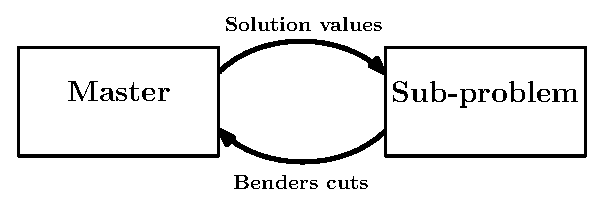
\includegraphics[width=0.6\textwidth]{images/bendersAbstract.eps}
\end{figure}

Since its introduction by \citeauthor{Benders1962},
this approach has been generalized to be applicable to a wider range of problem
structures. We now provide a review of the classical version of the method
as well as some of its recent adaptations.

\subsection{Classical Benders}
\label{sec:lit:clasBend}
The initial decomposition method proposed by \citeauthor{Benders1962}
was used to find the solutions of MIPs via partitioning
the problem into two simpler linear programs.
We refer the interested reader to the surveys by
\authciteb{Costa2005} and \authciteb{Rahmaniani2017}.
We now present how this decomposition could be applied
to a general minimization problem, based on the work
of \authciteb{Saharidis2010}.

Consider a problem where the set of decision variables
can be divided into two sets, $x$ and $y$, where
$y$ is a set of complicating variables.
The problem can be modelled by the following program
\begin{IEEEeqnarray}{rCl}
	\IEEEeqnarraymulticol{3}{c}{\text{Min }~ c^T x+d^T y}  \label{eq:lit:bendSimple1}\\[\eqnv]
	\text{s.t. }\quad Ax+By &\leq& b  \label{eq:lit:bendSimple2}\\[\eqnv]
	Fy &\leq& p    \label{eq:lit:bendSimple3}
\end{IEEEeqnarray}
By applying Benders decomposition here we receive
two simpler problems: a master deciding the $y$ variables with
all constraints involving $y$,
and a sub-problem deciding the $x$ variables with all
constraints involving $x$.
So by considering a trial solution, $y=\bar{y}$, of the complicating variables,
we can pass this information to the sub-problem
which is formulated as follow,
\begin{IEEEeqnarray}{rCl}
	\IEEEeqnarraymulticol{3}{c}{\text{Min }~ c^T x+d^T \bar{y}}  \label{eq:lit:bendSP1}\\[\eqnv]
	\text{s.t. }\quad Ax &\leq& b - B\bar{y}  \label{eq:lit:bendSP2}
\end{IEEEeqnarray}
Using the duality properties of LPs we can instead consider the
dual variables $u$ and represent this sub-problem by its dual as follows,
\begin{IEEEeqnarray}{rCl}
	\IEEEeqnarraymulticol{3}{c}{\text{Max }~ (b-B\bar{y})u } \label{eq:lit:bendSPdual1}\\[\eqnv]
	\text{s.t. }\quad A^T u &\leq& c  \label{eq:lit:bendSPdual2}
\end{IEEEeqnarray}
This is the sub-problem which is solved to optimality or
proven infeasible.
The objective function of the sub-problem varies with
$y$ but the feasible set of solutions is independent
of these complicating variables.

If the solution of the master problem is feasible
then the dual of the sub-problem will find optimality at 
an extreme point, while if the master's solution was
infeasible, the sub-problem is unbounded indicating the
existence of an extreme ray in its solution space.
In either case, we can formulate a Benders cut to add
back into the master problem to remove the current solution
from the feasible set.

When the sub-problem's solution is bounded and optimal
we can add what are called \emph{optimality} cuts to the master problem
\begin{IEEEeqnarray}{rCl}
	z&\geq& (b-By)\bar{u}_i^T + d^T y,\quad i=1,2,\ldots \label{eq:lit:bendExtPt}
\end{IEEEeqnarray}
where each $u_i$ corresponds to an extreme point. When the solution is unbounded
we can create \emph{feasibility} cuts for each extreme ray
\begin{IEEEeqnarray}{rCl}
	(b-By)\bar{v}_j^T &\leq& 0,\quad j=1,2,\ldots \label{eq:lit:bendExtRay}
\end{IEEEeqnarray}
where each $v_j$ corresponds to an extreme ray. After these cuts are created
we add them into the master problem and re-solve to find a new trial solution
for $y$. The new RMP is formulated as follows
\begin{IEEEeqnarray}{rClCl}
	\IEEEeqnarraymulticol{3}{c}{\text{Min }~ z} &\hspace{4mm}& \label{eq:lit:bendSimpleMast1}\\[\eqnv]
	\text{s.t. }\quad Fy &\leq& p & & \label{eq:lit:bendSimpleMast2}\\[\eqnv]
	z &\geq& (b-By)\bar{u}_i^T + d^T y & & i=1,2,\ldots   \label{eq:lit:bendSimpleMast3}\\[\eqnv]
	(b-By)\bar{v}_c^T &\leq& 0 & & j=1,2,\ldots   \label{eq:lit:bendSimpleMast4}
\end{IEEEeqnarray}

\authciteb{Geoffrion1972} generalized the classical approach to a broader class
of optimization problems which meant the sub-problems no longer needed
to be formulated as a linear program but could also be nonlinear.
Further to this improvement, \authciteb{Magnanti1981} investigated 
ways to generate Pareto-optimal Benders cuts to produce a tighter
relaxation in the master problem.
Other possible enhancement methods for Benders decomposition
exist including two- and three-phase heuristic approaches devised by \authciteb{Cordeau2001};
trust regions to significantly reduce the runtime considered by \authciteb{Santoso2005}
and \authciteb{Maher2014};
and parallelized solving of the decomposed problem studied by \authciteb{Dempster1998}
and \authciteb{Nielsen1997}.

\subsection{Logic-Based Benders}
\label{sec:lit:logicBend}
\citeauthor{Hooker2003}'s seminal paper from \citeyear{Hooker2003}
propose another generalization of Benders decomposition
to a much wider context while maintaining the strategy of
``learning from ones mistakes''.
One of the central ingredients in Benders decomposition
is the Benders cuts which allow information to be
communicated between the partitions of the problem.
In the classical case, the formulation of the sub-problems
is restricted to linear and non-linear programs.
However, this requirement hinders the ability of
Benders decomposition to be applied to problems
which are highly combinatorial in nature, such as scheduling,
as it can be impractical to formulate combinatorial problems
using a linear or non-linear model.

\citeauthor{Hooker2003} note that ``the key to generalizing Benders decomposition
is to extend the class of problems for which a suitable dual can be formulated''.
To this end, they introduced the concept of an \emph{inference dual} of any
optimization problem to the literature.
We note that this dual is different to the traditional LP dual
that the reader my be familiar with.
The inference dual is a proof of optimality which allows us to formulate
Benders cuts purely through logical reasoning.
This adaptation of the classical method proposed in \cite{Benders1962}
is named \emph{logic-based} Benders decomposition.

A formal description of logic-based Benders decomposition
applied to a minimization problem, based on the work
of \authciteb{Hooker2007}, is presented as follows.

Logic-based Benders decomposition applies to problems of the form
\begin{IEEEeqnarray}{rCl}
	\IEEEeqnarraymulticol{3}{c}{\text{Min }~ f(x,y)}  \label{eq:lit:bendLogicFormal1}\\[\eqnv]
	\IEEEeqnarraymulticol{3}{c}{\text{s.t. }\quad C(x,y)}   \label{eq:lit:bendLogicFormal2}\\[\eqnv]
	x &\in& D_x \label{eq:lit:bendLogicFormal3}\\[\eqnv]
	y &\in& D_y \label{eq:lit:bendLogicFormal4}
\end{IEEEeqnarray}
where $C(x,y)$ is a set of constraints depending on both the $x$ and $y$ variables.
General domains of $x$ and $y$ are denoted by $D_x$ and $D_y$ respectively.
If we consider fixing the value of $y$ to $\bar{y}\in D_y$, then
the following sub-problem arises
\begin{IEEEeqnarray}{rCl}
	\IEEEeqnarraymulticol{3}{c}{\text{Min }~ f(x,\bar{y})}  \label{eq:lit:bendLogicFormalSP1}\\[\eqnv]
	\IEEEeqnarraymulticol{3}{c}{\text{s.t. }\quad C(x,\bar{y})}   \label{eq:lit:bendLogicFormalSP2}\\[\eqnv]
	x &\in& D_x \label{eq:lit:bendLogicFormalSP3}
\end{IEEEeqnarray}
where $C(x,\bar{y})$ is the set of constraints that result by fixing $y=\bar{y}$.

The inference dual of the program (\ref{eq:lit:bendLogicFormalSP1}--\ref{eq:lit:bendLogicFormalSP3})
is the problem of inferring the tightest possible lower bound on $f(x,\bar{y})$ from $C(x,\bar{y})$.
Using the symbol ``$\Rightarrow$'' to denote logical implication, the
inference dual can be represented as follows
\begin{IEEEeqnarray}{rCl}
	\IEEEeqnarraymulticol{3}{c}{\text{Max }~ v} \label{eq:lit:bendLogicFormalSPdual1}\\[\eqnv]
	\text{s.t. }\quad C(x,\bar{y}) \overset{P}{\Rightarrow} f(x,\bar{y})&\geq& v  \label{eq:lit:bendLogicFormalSPdual2}\\[\eqnv]
	v &\in& \mathbb{R} \label{eq:lit:bendLogicFormalSPdual3}\\[\eqnv]
	P &\in& \mathcal{P} \label{eq:lit:bendLogicFormalSPdual4}
\end{IEEEeqnarray}
where $A\overset{P}{\Rightarrow} B$ means that $B$ can be deduced from $A$ via proof $P$
where $\mathcal{P}$ is a family of proofs.

The solution found by optimizing the inference dual can be interpreted
as a proof of the tightest possible bound, $\hat{v}$, on
$f(x,y)$ when $y$ is fixed to $\bar{y}$.
From this bound we derive a bounding function $B_{\bar{y}}(y)$
for other values of $y$.
The bounding function must satisfy two properties:
\begin{enumerate}
	\item[B1:] $B_{\bar{y}}(y)$ provides a valid lower bound on $f(x,y)$
	for any given $y\in D_y$. That is, $f(x,y)\geq B_{\bar{y}}(y)$ for
	any feasible $(x,y)$ in the program (\ref{eq:lit:bendLogicFormal1}--\ref{eq:lit:bendLogicFormal4}).
\item[B2:] In particular, $B_{\bar{y}}(\bar{y})=\hat{v}$.
\end{enumerate}
If we denote the objective function value of the program (\ref{eq:lit:bendLogicFormal1}--\ref{eq:lit:bendLogicFormal4})
by $z$ then the valid inequality $z\geq B_{\bar{y}}(y)$ is a Benders cut whose validity is proved
by the inference dual.

At the $\mu^{th}$ iteration of the Benders algorithm,
we solve the master problem with constraints defined
as the cuts generated so far
\begin{IEEEeqnarray}{rClCl}
	\IEEEeqnarraymulticol{3}{c}{\text{Min }~ z} &\hspace{4mm}& \label{eq:lit:bendLogicFormalRMP1}\\[\eqnv]
	\text{s.t. }\quad z &\geq& B_{y^h}(y) & & h=1,2,\ldots,\mu-1  \label{eq:lit:bendLogicFormalRMP2}\\[\eqnv]
	z &\in& \mathbb{R} & & \label{eq:lit:bendLogicFormalRMP3}\\[\eqnv]
	y &\in& D_y & &\label{eq:lit:bendLogicFormalRMP4}
\end{IEEEeqnarray}
where $y^1,\ldots,y^{\mu-1}$ are the previous solutions of the master problem.
The solution $\bar{y}$ of the $\mu^{th}$ master %, \ie program (\ref{eq:lit:bendLogicFormalRMP1}--\ref{eq:lit:bendLogicFormalRMP4}),
defines the next sub-problem to be solved.

We denote $v_1^*,\ldots,v_{\mu-1}^*$ as the optimal values of the previous $\mu-1$ sub-problems.
The algorithm continues to iterate between
the master and sub-problem until the optimal value $z_\mu^*$
of the master equals $v^*=\min\{v_1^*,\ldots,v_{\mu-1}^*\}$.

% In Figure \ref{fig:lit:topLevelBendersFlowchart}, we provide
% a flowchart detailing the execution of logic-based Benders decomposition.
% We advise the reader to take this as only a framework
% of the process rather than an exact step-by-step method,
% as it's generality makes it well-suited
% to a number of modifications.
% \begin{figure}[tbp]
% 	\centering
% 	\caption{High level flowchart of logic-based Benders decomposition}
% 	\label{fig:lit:topLevelBendersFlowchart}
% 	\includegraphics[width=0.5\textwidth]{images/noimg.png}
% \end{figure}

This new decomposition method allows the general strategy
of Benders decomposition to be applied to a much wider class
of problems, however using the logic-based version
means that for each problem a new method of generating Benders
cuts needs to be devised.
Further to this, each new Benders cut must be rigorously 
proven to be valid, \ie not remove any possibly optimal
solution from the solution space.
In the classical case, this formal proof was not
expressly required as the validity of any cut was
confirmed by the duality theory of linear programming.

\subsection{Hybrid-Benders}
\label{sec:lit:hybridBend}
To illustrate the benefits that employing logic-based Benders decomposition
can provide, we detail one of its a special cases which has demonstrated success in
the literature: hybrid Benders decomposition.
What distinguishes the hybrid variant
is the use of multiple kinds of solving technology
to tackle a single problem
within a logic-based Benders decomposition framework.

Here we will examine examples from the literature
where MIP solvers were effectively combined with CP solvers
to take advantage of their complimentary strengths.
The benefits of employing such an approach are clear when the
structure of a problem allows a natural decomposition,
and the resulting partitions can each be efficiently
solved by different kinds of solvers.
MIP solvers have been successfully applied to solve a wide
range of problems including network synthesis,
crew scheduling, planning and capital budgeting.
While the FD propagation of CP solvers has been effectively
applied to solve combinatorial discrete optimization problems
and feasibility problems for resource allocation and scheduling.

\authciteb{Jain2001} considered a parallel machine sequencing problem
and devised a Benders decomposition of the original problem into a set of assignment decisions
and a set of sequencing decisions.
A MIP model was devised to tackle the assignment problem, 
which could take advantage of the LP relaxation and
\bab search offered by MIP solvers.
Testing the feasibility of the solutions of the relaxed problem
could be achieved efficiently by making use of the propagation
engines offered by CP solvers.
The feasibility sub-problems were linked to the assignment master problem
via a set of feasibility Benders cuts.
In their case, multiple nogood cuts were generated
at each iteration of the Benders algorithm.

The complimentary strengths between MIP and CP solvers
have been noted by \authciteb{Timpe2002}, \authciteb{Benoist2002} 
and \authciteb{Hooker2005}.
The problems tackled by these papers
demonstrate the wide applicability of this framework.
Specifically these authors approached the
following problems: polypropylene batch scheduling,
call centre scheduling and multi-machine scheduling respectively.

\authciteb{Li2009a} use the hybrid Benders decomposition
framework to model a variant of the well-studied
Resource Constrained Project Scheduling Problem (\RCPSP).
The \RCPSP is a highly combinatorial optimization problem 
with a number of extensions in the literature \cite{Szeredi2016,Tran2012}.
This scheduling problem is naturally suited to be modelled
by the global constraints \cumu and \disj offered by CP.
Due to this, a number of advances have been made in theory
of CP solvers to improve their ability to solve the \RCPSP.
Some of these advances were detailed previously
in Section \ref{sec:lit:cp}.

The variant considered by \citeauthor{Li2009a}
introduces an additional layer of complexity to the problem
by allowing each of the resources to have more than just 
a singular capability, as is the case in the basic \RCPSP.
This addition results in a set of assignment decisions
between the resources and the tasks of the project.
As the problem now had two distinct sets of decisions ---
assignment and scheduling --- they chose to employ
a Benders decomposition.
The consequence was a relaxed master problem, modelled as a MIP
to handle the assignment decisions and a feasibility sub-problem
encoded as a constraint program.
As a result of this decomposition, \citeauthor{Li2009a} were still able to utilize the 
global constraints of CP to effectively encode the scheduling aspect of the problem.
The authors' hybrid Benders decomposition is notable
due to the variety of both optimality and feasibility
Benders cuts they were able to formulate.
In their further work \cite{Li2009b,Li2012,Li2015} a number of
problems involving assignment and scheduling decisions
are tackled again using this hybrid approach to achieve
an effective decomposition.

\authciteb{Tran2012} consider another variant of the \RCPSP,
closely related to the assembly line balancing
problem we are concerned with in this thesis.
Specifically, their focus was on the resource constrained scheduling problem
with unrelated machines and sequence-dependent setup times between tasks.
They applied a logic-based Benders decomposition and formulated
a hybridized solution methodology.
Their decomposition of the problem gave them the
ability to formulate each sub-problem as an asymmetric TSP.
The TSP is a combinatorial optimization problem which is of
particular interest to the academic community and as such,
dedicated solvers which are tailored to this problem
are available \cite{Applegate2017}.
Having the ability to take advantage of the wealth of 
research into the inherent combinatorial sub-structure of their problem,
the TSP, allowed their method to solve problems
six orders of magnitude faster than what was previously possible
by MIP solvers, while also allowing the optimal solution
to be found for instances twice as large as previously able.

\subsection{Summary}
We hope these applications of logic-based Benders decomposition
to a range of difficult problems has provided
some insight into this framework's applicability.
When problems can naturally be decomposed into their more basic
combinatorial components, it is possible to achieve superior
results by combining solution approaches which can more readily
exploit the inherent structures of the problem.